%-----------------------------------------------------------------------------------------------------------------------------------------------%
%	The MIT License (MIT)
%
%	Copyright (c) 2015 Jan Küster
%
%	Permission is hereby granted, free of charge, to any person obtaining a copy
%	of this software and associated documentation files (the "Software"), to deal
%	in the Software without restriction, including without limitation the rights
%	to use, copy, modify, merge, publish, distribute, sublicense, and/or sell
%	copies of the Software, and to permit persons to whom the Software is
%	furnished to do so, subject to the following conditions:
%	
%	THE SOFTWARE IS PROVIDED "AS IS", WITHOUT WARRANTY OF ANY KIND, EXPRESS OR
%	IMPLIED, INCLUDING BUT NOT LIMITED TO THE WARRANTIES OF MERCHANTABILITY,
%	FITNESS FOR A PARTICULAR PURPOSE AND NONINFRINGEMENT. IN NO EVENT SHALL THE
%	AUTHORS OR COPYRIGHT HOLDERS BE LIABLE FOR ANY CLAIM, DAMAGES OR OTHER
%	LIABILITY, WHETHER IN AN ACTION OF CONTRACT, TORT OR OTHERWISE, ARISING FROM,
%	OUT OF OR IN CONNECTION WITH THE SOFTWARE OR THE USE OR OTHER DEALINGS IN
%	THE SOFTWARE.
%	
%
%-----------------------------------------------------------------------------------------------------------------------------------------------%


%============================================================================%
%
%	DOCUMENT DEFINITION
%
%============================================================================%

%we use article class because we want to fully customize the page and dont use a cv template
\documentclass[10pt,A4]{article}	


%----------------------------------------------------------------------------------------
%	ENCODING
%----------------------------------------------------------------------------------------

%we use utf8 since we want to build from any machine
\usepackage[utf8]{inputenc}		

%----------------------------------------------------------------------------------------
%	LOGIC
%----------------------------------------------------------------------------------------

% provides \isempty test
\usepackage{xifthen}

%----------------------------------------------------------------------------------------
%	FONT
%----------------------------------------------------------------------------------------

% some tex-live fonts - choose your own

%\usepackage[defaultsans]{droidsans}
%\usepackage[default]{comfortaa}
%\usepackage{cmbright}
\usepackage[default]{raleway}
%\usepackage{fetamont}
%\usepackage[default]{gillius}
%\usepackage[light,math]{iwona}
%\usepackage[thin]{roboto} 

% set font default
\renewcommand*\familydefault{\sfdefault} 	
\usepackage[T1]{fontenc}

% more font size definitions
\usepackage{moresize}		


%----------------------------------------------------------------------------------------
%	PAGE LAYOUT  DEFINITIONS
%----------------------------------------------------------------------------------------

%debug page outer frames
%\usepackage{showframe}			

%define page styles using geometry
\usepackage[a4paper]{geometry}		

% for example, change the margins to 2 inches all round
\geometry{top=1.25cm, bottom=-.6cm, left=1.5cm, right=1.5cm} 	

%use customized header
\usepackage{fancyhdr}				
\pagestyle{fancy}

%less space between header and content
\setlength{\headheight}{-5pt}		

%customize entries left, center and right
%\lhead{}
%\chead{}
%\rhead{}

%indentation is zero
\setlength{\parindent}{0mm}

%----------------------------------------------------------------------------------------
%	TABLE /ARRAY DEFINITIONS
%---------------------------------------------------------------------------------------- 

%for layouting tables
\usepackage{multicol}			
\usepackage{multirow}

%extended aligning of tabular cells
\usepackage{array}

\newcolumntype{x}[1]{%
>{\raggedleft\hspace{0pt}}p{#1}}%


%----------------------------------------------------------------------------------------
%	GRAPHICS DEFINITIONS
%---------------------------------------------------------------------------------------- 

%for header image
\usepackage{graphicx}

% for GitHub/Linkdin/... icons 
\usepackage{fontawesome}

% for hyper links
\usepackage{hyperref}

%for floating figures
\usepackage{wrapfig}
\usepackage{float}
%\floatstyle{boxed} 
%\restylefloat{figure}

%for drawing graphics		
\usepackage{tikz}				
\usetikzlibrary{shapes, backgrounds,mindmap, trees}


%----------------------------------------------------------------------------------------
%	Color DEFINITIONS
%---------------------------------------------------------------------------------------- 

\usepackage{color}

%accent color
\definecolor{sectcol}{RGB}{0,150,255}

%dark background color
\definecolor{bgcol}{RGB}{110,110,110}

%light background / accent color
\definecolor{softcol}{RGB}{225,225,225}


%============================================================================%
%
%
%	DEFINITIONS
%
%
%============================================================================%

%----------------------------------------------------------------------------------------
% 	HEADER
%----------------------------------------------------------------------------------------

% remove top header line
\renewcommand{\headrulewidth}{0pt} 

%remove botttom header line
\renewcommand{\footrulewidth}{0pt}	  	

%remove pagenum
\renewcommand{\thepage}{}	

%remove section num		
\renewcommand{\thesection}{}			

%----------------------------------------------------------------------------------------
% 	ARROW GRAPHICS in Tikz
%----------------------------------------------------------------------------------------

% a six pointed arrow poiting to the left
\newcommand{\tzlarrow}{(0,0) -- (0.2,0) -- (0.3,0.2) -- (0.2,0.4) -- (0,0.4) -- (0.1,0.2) -- cycle;}	

% include the left arrow into a tikz picture
% param1: fill color
%
\newcommand{\larrow}[1]
{\begin{tikzpicture}[scale=0.58]
	 \filldraw[fill=#1!100,draw=#1!100!black]  \tzlarrow
 \end{tikzpicture}
}

% a six pointed arrow poiting to the right
\newcommand{\tzrarrow}{ (0,0.2) -- (0.1,0) -- (0.3,0) -- (0.2,0.2) -- (0.3,0.4) -- (0.1,0.4) -- cycle;}

% include the right arrow into a tikz picture
% param1: fill color
%
\newcommand{\rarrow}
{
\begin{tikzpicture}[scale=0.7]
	\filldraw[fill=sectcol!100,draw=sectcol!100!black] \tzrarrow
 \end{tikzpicture}
}



%----------------------------------------------------------------------------------------
%	custom sections
%----------------------------------------------------------------------------------------

% create a coloured box with arrow and title as cv section headline
% param 1: section title
%
\newcommand{\cvsection}[1]
{
	\begin{center}
		\large\textcolor{sectcol}{\textbf{#1}}
	\end{center}
}

%create a coloured arrow with title as cv meta section section
% param 1: meta section title
%
\newcommand{\metasection}[2]
{
%\begin{tabular*}{1\textwidth}{r r}
\footnotesize{#2} \hspace*{\fill} \footnotesize{#1}\\[1pt]
%\end{tabular*}
}

%----------------------------------------------------------------------------------------
%	 CV EVENT
%----------------------------------------------------------------------------------------

% creates a stretched box as cv entry headline followed by some paragraphs about 
% the work you did
% param 1:	event time i.e. 2014 or 2011-2014 etc.
% param 2:	event name (what did you do?)
% param 3:	institution (where did you work / study)
% param 4:	list of paragraphs
%
\newcommand{\cvevent}[5]
{

\begin{tabular*}{1\textwidth}{p{13.6cm} x {3.9cm}}
	\textbf{#2} - \textcolor{bgcol}{#3} &  \vspace{2pt}\textcolor{sectcol}{#1}
\end{tabular*}

\vspace{-8pt}
\textcolor{softcol}{\hrule}

\vspace{6pt}{#4}
\vspace{6pt}

\ifthenelse{\isempty{#5}}{}{
    \foreach \desc in {#5}{
        $\cdot$ \desc\\[3pt]
    }%
}
	
\vspace{3pt}
}

% creates a stretched box as 
\newcommand{\cveventmeta}[2]
{
	\mbox{\mystrut \hspace{87pt}\textit{#1}}\\
	#2
}

%----------------------------------------------------------------------------------------
% CUSTOM STRUT FOR EMPTY BOXES
%----------------------------------------- -----------------------------------------------
\newcommand{\mystrut}{\rule[-.3\baselineskip]{0pt}{\baselineskip}}

%============================================================================%
%
%
%
%	DOCUMENT CONTENT
%
%
%
%============================================================================%
\begin{document}

%use our custom fancy header definitions
\pagestyle{fancy}	

%---------------------------------------------------------------------------------------
%	PHOTO and TITLE HEADLINE
%----------------------------------------------------------------------------------------
\vspace{-8pt}

\begin{minipage}{0.8\textwidth}\flushleft
    \HUGE \textsc{MING-RUEY(RAY) CHOU}\\[2pt]
	\small Computer Vision Engineer
\end{minipage}
\begin{minipage}{0.2\textwidth}\flushright
    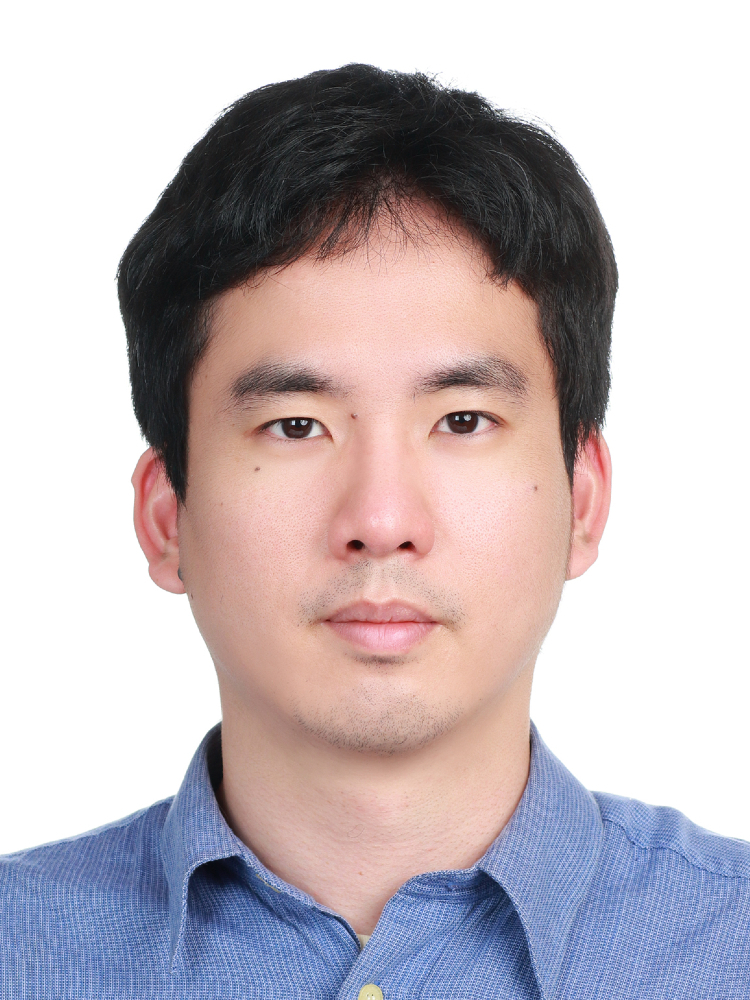
\includegraphics[scale=0.04,trim={0 8cm 0 0},clip]
    {./photo.jpg}
\end{minipage}

\vspace{6pt}

%---------------------------------------------------------------------------------------
%	META SECTION
%----------------------------------------------------------------------------------------
\metasection{Taipei, Taiwan}{Fields: Image processing algorithm devlopement and optimization}
\metasection{\faicon{envelope} imchou239@gmail.com}{Tools \& Libraries: OpenCV, Tensorflow, Jax, Docker, Git}
\metasection{\faicon{github} MingRuey}{Programming Languages: Python, C\#, C{++}, CUDA}
\metasection{\faicon{linkedin} ---}{}
\vspace{-2pt}
\textcolor{softcol}{\hrule}
\vspace{6pt}

\normalsize

%---------------------------------------------------------------------------------------
%	SUMMARAY (optional)
%----------------------------------------------------------------------------------------
\vspace{-6pt}
\cvsection{Summary}
Digital media graduate with project experience in the field of technology based assessment. Currently working as IT Consultant at We4IT, Bremen in the field of IBM Notes Domino and XPages applications. Master studies focused on teams from different disciplines and cultural backgrounds on solutions for complex problems.\\


%============================================================================%
%
%	CV SECTIONS AND EVENTS (MAIN CONTENT)
%
%============================================================================%

%---------------------------------------------------------------------------------------
%	EXPERIENCE
%----------------------------------------------------------------------------------------
\cvsection{Experience}

\cvevent
    {2021 JUL - Current}{Machine Learning Engineer}
    {Geosciences of Princeton University, NJ, USA}
    {GGGG}{
    {\href{https://www.cylai.princeton.edu/}{Lai Research Group}},
	{Develop and evaluate the next generation learning management system with Meteor}
}

\cvevent
    {2019 - 2021 JUN}{Computer Vision Engineer}
    {\href{https://www.utechzone.com.tw/index_en.php}{UTECHZONE}, Taipei, Taiwan}
    {GGG}{
	{Develop and evaluate the next generation learning management system with Meteor},
	{Develop and evaluate the next generation learning management system with Meteor}
}

%---------------------------------------------------------------------------------------
%	EDUCATION SECTION
%--------------------------------------------------------------------------------------
\cvsection{Education}

\cvevent
    {2016}{M.Sc. in Physics}
    {National Taiwan University}
    {GG}{
	{Thesis: Rheometry on Concentrated Suspension of Soft Particles},
    {\href{https://doi.org/10.1039/D0SM00405G}{Publish on Soft Matter: doi.org/10.1039/D0SM00405G}},
    {\href{http://www.phys.sinica.edu.tw/jctsai/Ray2016/}{Mandarin website: www.phys.sinica.edu.tw/jctsai/Ray2016/}}
}

\cvevent
    {2013}{B.Sc. in Physics}
    {National Taiwan University}
    {}{
}

%---------------------------------------------------------------------------------------
%	OTHERS SECTION
%--------------------------------------------------------------------------------------
\cvsection{Other Experience}

\cvevent
    {2018 to Present}{Course Design and Project Mentor}
    {Twin Oaks}
    {}{
}
\cvevent
    {2017}{Substitute Services in Education}
    {Xinyi Elementary School, Hualien Taiwan}
    {}{
}

%--------------------------------------------------------------------------------------------------
%	ARTIFICIAL FOOTER (fancy footer cannot exceed linewidth) 
%--------------------------------------------------------------------------------------------------

% \null
% \vspace*{\fill}
% \hspace{-0.25\linewidth}\colorbox{white}{}


%============================================================================%
%
%
%
%	DOCUMENT END
%
%
%
%============================================================================%
\end{document}
